\documentclass[border=4pt]{standalone}

\usepackage{amsmath}
\usepackage{tikz}
\usepackage{mathdots}
\usepackage{yhmath}
\usepackage{cancel}
\usepackage{color}
\usepackage{siunitx}
\usepackage{array}
\usepackage{multirow}
\usepackage{amssymb}
\usepackage{gensymb}
\usepackage{tabularx}
\usepackage{booktabs}
\usetikzlibrary{fadings}
\usetikzlibrary{patterns}


\begin{document}
 
 \tikzset{every picture/.style={line width=0.75pt}} %set default line width to 0.75pt

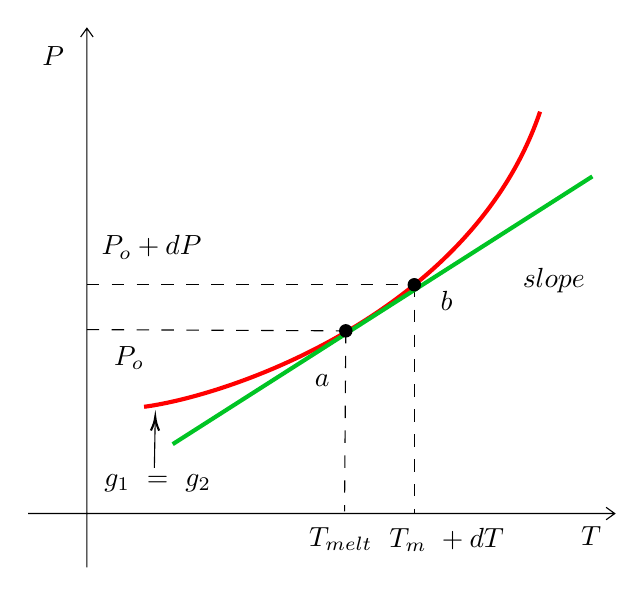
\begin{tikzpicture}[x=0.75pt,y=0.75pt,yscale=-0.6,xscale=0.6]
%uncomment if require: \path (0,433); %set diagram left start at 0, and has height of 433

%Shape: Axis 2D [id:dp34042133393206886]
\draw  (72,390.7) -- (543,390.7)(119.1,1) -- (119.1,434) (536,385.7) -- (543,390.7) -- (536,395.7) (114.1,8) -- (119.1,1) -- (124.1,8)  ;
%Straight Lines [id:da6702336744569144]
\draw  [dash pattern={on 4.5pt off 4.5pt}]  (327,244) -- (326,389) ;


%Straight Lines [id:da7053989083670136]
\draw  [dash pattern={on 4.5pt off 4.5pt}]  (382,207) -- (382,390) ;


%Curve Lines [id:da6886563534922254]
\draw [color={rgb, 255:red, 255; green, 0; blue, 0 }  ,draw opacity=1 ][line width=1.5]    (165,305) .. controls (239,295) and (429,227) .. (483,68) ;


%Straight Lines [id:da01620685432223168]
\draw  [dash pattern={on 4.5pt off 4.5pt}]  (119,243) -- (327,244) ;


%Straight Lines [id:da6787352217788557]
\draw  [dash pattern={on 4.5pt off 4.5pt}]  (119,207) -- (382,207) ;


%Straight Lines [id:da3303084254473059]
\draw [color={rgb, 255:red, 0; green, 196; blue, 36 }  ,draw opacity=1 ][line width=1.5]    (188,335) -- (525,120) ;


%Shape: Circle [id:dp23372095277787042]
\draw  [color={rgb, 255:red, 0; green, 0; blue, 0 }  ,draw opacity=1 ][fill={rgb, 255:red, 0; green, 0; blue, 0 }  ,fill opacity=1 ] (377.05,207) .. controls (377.05,204.26) and (379.26,202.05) .. (382,202.05) .. controls (384.74,202.05) and (386.95,204.26) .. (386.95,207) .. controls (386.95,209.74) and (384.74,211.95) .. (382,211.95) .. controls (379.26,211.95) and (377.05,209.74) .. (377.05,207) -- cycle ;
%Shape: Circle [id:dp06058395143705542]
\draw  [color={rgb, 255:red, 0; green, 0; blue, 0 }  ,draw opacity=1 ][fill={rgb, 255:red, 0; green, 0; blue, 0 }  ,fill opacity=1 ] (322.05,244) .. controls (322.05,241.26) and (324.26,239.05) .. (327,239.05) .. controls (329.74,239.05) and (331.95,241.26) .. (331.95,244) .. controls (331.95,246.74) and (329.74,248.95) .. (327,248.95) .. controls (324.26,248.95) and (322.05,246.74) .. (322.05,244) -- cycle ;
%Straight Lines [id:da4596906688697088]
\draw    (173.28,353.97) -- (173.96,315.12) ;
\draw [shift={(174,313.12)}, rotate = 451] [color={rgb, 255:red, 0; green, 0; blue, 0 }  ][line width=0.75]    (10.93,-3.29) .. controls (6.95,-1.4) and (3.31,-0.3) .. (0,0) .. controls (3.31,0.3) and (6.95,1.4) .. (10.93,3.29)   ;


% Text Node
\draw (92,23) node   {$P$};
% Text Node
\draw (524,409) node   {$T$};
% Text Node
\draw (323,411) node   {$T_{melt}$};
% Text Node
\draw (408,412) node   {$T_{m} \ +dT$};
% Text Node
\draw (153,266) node   {$P_{o}$};
% Text Node
\draw (171,177) node   {$P_{o} +dP$};
% Text Node
\draw (308,284) node   {$a$};
% Text Node
\draw (408,220) node   {$b$};
% Text Node
\draw (494,204) node   {$slope$};
% Text Node
\draw (176,366.2) node   {$g_{1} \ =\ g_{2}$};


\end{tikzpicture}

\end{document}
